\section{Introduction}
Climate change, extreme weather, and the state of the environment directly impact the availability of food~\cite{akil2014effects},~\cite{RW3}, energy~\cite{mitigation2011ipcc}, and shelter~\cite{warner2009search}.
As finite resources become scarce, the residual impacts on local economies can have disastrous and long-lasting effects on the fundamental livelihoods of inhabitants for decades~\cite{le2001political}.
The examples of this occurring are numerous.
The extended drought in Syria in 2011 is cited as one of the principle causes of civil war \cite{gleick2014water,kelley2015climate}.
In a smaller scale example, the environmental impact of lead contamination in the drinking water in the United States led to protests in 2016.
The extreme weather event, Hurricane Manuel, that devastated the western coasts of Mexico led to subsequent protests over resources at points as long as 1 year after the initial event.

Of course, the occurrence of either a shift in climate, extreme weather, or environmental catastrophe is not sufficient to guarantee that civil unrest is likely to follow.
In general the causal mechanisms leading to civil unrest are very complex, and there is no easy way to determine a linear pathway to protest.
However, to date, little quantitative analysis has been performed on the residual effects of changes resulting from climate, extreme weather, and the environment using a large volume of data.
In this analysis, we focus on the breadth of the climate events by looking at events generated from a large Gold Standard Report (GSR) containing all of the protests that have occurred in Latin America from 2011-2015.

GSR is a gold standard report of protests organized by MITRE, using human analysts, to survey newspapers for reportings of civil unrest. The GSR includes many features, as shown in Figure~\ref{GSR}, such as protest location, event date, protest type, status, crowd size, headline, date, population, protest description, first reported links, etc.. The description feature is brief description of the protest, generally, it tells us who, where, why and when protest. As Figure~\ref{GSR} shows, the protest description is `small farmers want the bank to forgive their debts due to the drought, which has hampered production'.

\begin{figure}[th]
\centerline
{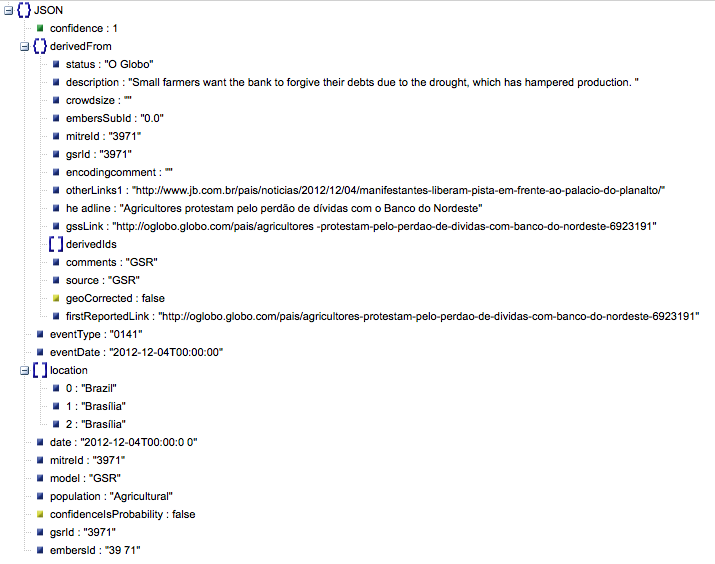
\includegraphics[width = 4in]{figures/gsr_event_json.png}}
\caption{Gold standard report (GSR) format.}
\label{GSR}
\end{figure}

We address three foundational problems: first, the identification of climate related protest. By developing a logistic regression classifier, 25352 GSR civil unrest events were classified as either being climate or non-climate related using terms in the description of the event. Second, from analyzing large historical climate protests records, we look into the text description of protests and extract the climate protest category for each country. For each major climate category, we adopt the knowledge graph approach to define linkage relationship between entities, and study the possible protest causalities. Third, we find that the massive climate protests have coherent correlations within them, we also show that certain protest types are more prone to associate with certain other protest types, such as lack of water is highly linked with power shortage, and so on. Generally, the main contribution of this paper can be summarized as:

\begin{enumerate}
  \item We develop a logistic regression classifier, which can classify climate protests from non-climate protests automatically based on protest event descriptions.
  \item We analyze the climate protest spikes and disclose its relationship with climate disasters. For instance, the time span caused by storm and hurricane events in Mexico last much longer. However, for drought events in Brazil, the protests being initiated more swiftly, also last much shorter.
  \item We figure out the proportion of protest causality. By studying some major climate disasters, we also discover each protest category's evolution pattern, thus how does the climate disasters lead to armed climate protests.
  \item We investigate the climate co-occurrence. For instance, the water related protests are often accompanies with electricity shortage, while land ownership protests are often associate with farmers.
\end{enumerate}
%

\section{Related research}
The path from climate, extreme weather and environmental effects to civil unrest is causally complex \cite{hsiang2011civil,RW5} and involves various combinations of climate change \cite{burke2014climate}, natural resources, human security, and social stability.
In general, sensitivities to climate change, exposure to climate change, and the ability of a society to adapt are indicators of whether or not violence will erupt~\cite{RW9}.
A commonly studied pathway is the effect of climate on food prices which then induces civil unrest.
An examples of this occurrence is the Arab Spring uprisings in 2011, and how weather effects food prices~\cite{RW2}.
The pathway to civil unrest is also not limited to a local region, where one study shows the Chinese drought effecting the supply wheat causing prices to rise in the Egyptian break market leading to protest~\cite{RW1}.
The pathways of food prices to protest have also been studied in the global south~\cite{RW4}, Africa, and Asia~\cite{wischnath2014climate,RW6}.
However, even this path of climate effects on income level leading to conflict is not eminently clear~\cite{RW10}.


\section{Climate protest classifier}
The classifier is designed to label text documents into two or more predefined categories. In this work, we only have two categories: climate or non-climate related protest. By sample analysis, more than 90\% records belongs to non-climate related protest, thus the dataset can be ascribed as un-balanced dataset. So we consider majority assign classification as baseline, adopt other four classical classification methods: K-Nearest Neighbor, Naive Bayes, weighted SVM and Logistic regression.

%Text classification is a process of grouping text documents into one or more predefined categories based on their content. The first step in text categorization is to transform documents, which typically are strings of characters, into a representation suitable for the learning algorithm and the classification task. The most commonly used document representation is the so-called vector space model. In this model, each document is represented by a vector of words.

\subsection{Majority assign}
Majority assign method is taken as a baseline for the unbalanced classification dataset. It first calculates the climate related protest rate with the training data-set as $p$, and non-climate related protest as $1-p$, and then uses this distribution to randomly assign each testing event. Suppose there are $N$ testing events, by this algorithms, the true-positive would be $Np^2$, false-positive and false-negative would both be $Np(1-p)$, on average. Hence the precision, recall and $F-measure$ would all be $p$, and the accuracy would be $p^2+(1-p)^2$. For unbalanced data-set, since $p<<(1-p)$, the accuracy approximately equals to $(1-p)^2$, while the $F-measure$ is $p$.

\subsection{K Nearest Neighbor}
To classify a class-unknown document X, the K-Nearest Neighbor (KNN) classifier algorithm ranks the document's neighbors among the training document vectors, and uses the class labels of the k most similar neighbors to predict the class of the new document. The classes of these neighbors are weighted using the similarity of each neighbor to X, where similarity is measured by Euclidean distance or the cosine value between two document vectors~\cite{liao2002using}.

KNN has been used in statistical estimation and pattern recognition already in the beginning of 1970�s as a non-parametric technique.  A case is classified by a majority vote of its neighbors, with the case being assigned to the class most common amongst its K nearest neighbors measured by a distance function. If K = 1, then the case is simply assigned to the class of its nearest neighbor. Choosing the optimal value for K is best done by first inspecting the data. We first manually identify 100 climate-related protest events as the training sets. In our protest filter design, text similarity measures play a fundamentally important, where apply Corpus-Based similarity for distance computation between different event descriptions. In our experiment, we set K to be 100.

\subsection{Naive Bayes}
Essentially, Naive Bayes is maximum a posteriori classifier, which can be represented as $c = \mathrm{argmax}_c{p(c|e)}$. $e$ is the protest description, and consists of multiple words $w_i$, and can be denoted as $e=<w_0, w_1,...>$. $c=\{climate protest, non-climate protest\}$. However, there is no trivial solution to measure the joint probability distribution for $e,c$ considering the extremely complex underlying structures among $w_i$. Naive Bayes circumvents this problem by assuming the independency among $w_i$. Hence, the probability of each protest $e$ being class $c$ can be simplified as: $$p(c|e)\propto p(c)\prod_i p(w_i|c)$$, where $p(w_i|c)=\frac{f_{w_i}^c}{f_{w}^c}$ is the conditional probability of term $w_i$ that appears in the description of $e$. $f_{w_i}^c$ is the occur frequencies of $w_i$ in class $c$, and $f_{w}^c$ is the total word number in class $c$.  If a new term $w_i$ does not occur in the training dataset, then $p(w_i|c) = 0$. $p(w_i|c)$ measures how much likeness of being $c$ for the existence of term $w_i$. To mitigate the zeroing affects, $Laplace-smoothing$ modifies $p(w_i|c)$ as $$p(w_i|c)=\frac{f_{w_i}^c+1}{f_{w}^c+W}$$, where $W$ is the total word number for climate and non-climate protests together. Usually, the conditional probability is small which might results in float point underflow. In reality, it is converted as: $$c = \mathrm{argmax}{p(c|e)}=\mathrm{argmax}_c\{log(p(c)) + \sum_ilog(p(w_i)|c)\}.$$


\subsection{Weighted Support Vector Machine}
The training data consists of $N$ pairs $(x_1,y_1),(x_2,y_2),...,(x_N,y_N)$, with $x_i\in \mathbb{R}^p$, and $y_i \in \{-1,+1\}$. By the introducing a hyperplane of $P:=\{x| x^T\beta+\beta_0=0\}$, the classification rule is defined as $G(x)=\text{sign}[x^T\beta+\beta_0].$To find the hperplane $P$ for unseperable sets, it is often converted into the following quadratic convex optimization problem by defining the slack variables $\zeta=(\zeta_1,\zeta_2,..,\zeta_N)$.

\begin{equation}
    \label{eq:svm}
    \begin{aligned}
& \underset{\beta, \beta_0}{\text{minimize}}
    & & \frac 1 2||\beta||^2 +C \sum_{i=1}^N \zeta_i \\
    & \text{subject to}
        & & y_i(x_i^T\beta+\beta_0) \ge 1-\zeta_i,&\forall i  \\
        & & & \zeta_i \ge 0, &\forall i \\
    \end{aligned}
\end{equation}
$C$ is the penalty parameter. For separable sets, $C$ corresponds to $\infty$.\\The problem with above classifer is that the penalty for misclassification are the same. However, there are a lot of cases the miss alram should have a much higher cost than the false alarms. To considet those scenarios, we introduce two different penalty for miss alarm and false alarm. For simplicity, $I$ and $J$ denotes the subscript of positive and negative set. Thus, the problem of \ref{eq:svm} can be re-formulated as:

\begin{equation}
\label{eq:svm2}
\begin{aligned}
    & \underset{\beta, \beta_0}{\text{minimize}} & \frac 1 2||\beta||^2 + C_1 \sum_{i\in I} \zeta_i + C_2 \sum_{j\in J} \eta_j \\
    & \text{subject to} & x_i^T\beta+\beta_0 \ge 1-\zeta_i,&\forall i \in I  \\
      & & x_j^T\beta+\beta_0 \leq -1+\eta_j,&\forall j \in J  \\
      && \zeta_i \ge 0,&\forall i \in I  \\
      && \eta_j \ge 0,&\forall j \in J  \\
\end{aligned}
\end{equation}

The Lagrange function of \ref{eq:svm2} is

\begin{equation}
\label{eq:svm2}
\begin{aligned}
    L_p =&  \frac 1 2||\beta||^2 + C_1 \sum_{i\in I} \zeta_i + C_2 \sum_{j\in J} \eta_j\\
        &-\sum_{i \in I}\alpha_i[x_i^T\beta+\beta_0- (1-\zeta_i)]-\sum_{i \in I}\mu_i\zeta_i\\
        &+\sum_{j \in J}\theta_j[x_j^T\beta+\beta_0- (1-\eta_j)]-\sum_{j \in J}\tau_j\eta_j\\
\end{aligned}
\end{equation}



The input of the SVM experiment is GSR json file, and the input file includes lots of features. Among these features, several of them are more important than others, including status, description, crowdsize, headline, eventType, eventDate, location, date, population etc. The description feature is brief description of the events, which plays a dominant role in the entire dataset.

In order to apply SVM algorithm on GSR dataset, we need to vectorize text data in the dataset. First of all, we construct a word corpus which includes every word shown in the dataset (including non-words). We accept non-words because most coinages come from Internet and some of them might be important for the events. As we accept non-words, the corpus might be large than our corpus vocabulary. Then, for every fields, the content is converted to a corresponding vector based on the corpus. If one word exists in specific field, a calculated value will be assign to the corresponding element in the vector. Other numerical values will also be added in the vector. By this way, we could convert the dataset into a huge matrix.

Minimizing (2) can be rewritten as a constrained optimization problem with a differentiable objective function in the following way.

For each $i \in \{1,\,\ldots,\,n\}$ we introduce the variable $\zeta_i$, and note that $ \zeta_i = \max\left(0, 1 - y_i(w\cdot x_i + b)\right)$  if and only if $ \zeta_i$ is the smallest nonnegative number satisfying $ y_i(w\cdot x_i + b) \geq 1- \zeta_i.$

Thus we can rewrite the optimization problem as follows$$ \text{minimize } \frac 1 n \sum_{i=1}^n \zeta_i + \lambda\|w\|^2 $$, $$ \text{subject to } y_i(x_i \cdot w + b) \geq 1 - \zeta_i \,\text{ and }\,\zeta_i \geq 0,\,\text{for all }i.$$This is called the ''primal'' problem.After the preprocessing, we could apply SVM algorithm on GSR matrix. We randomly label 1000 events from GSR dataset and use ten-fold cross validation to train out SVM. Figure 1 shows the result of SVM experiment.


\subsection{Logistic regression classifier}
From GSR events, we devised a climate protest classifier to identify the climate related protest events automatically. The classifier is built based on logistic regression model. With input of GSR descriptions, we aim to train a classifier which can label a protest description as climate related or not. The GSR includes many potential important features, such as status, description, crowd size, headline, event Type, event Date, location, date, population etc. The description feature is brief description of the events, which plays a dominant role in the entire dataset. In order to adopt logistic regression on GSR dataset, we need to vectorize text data in the dataset. First of all, we construct a word corpus which includes every word $x_i$ shown in the training dataset (including non-words). We accept non-words because most coinages come from Internet and some of them might be important for the events. As we accept non-words, the corpus might be large than our corpus vocabulary. The word corpus is composed with $[x_1, x_2, ..., x_i, ..., x_N]$.
Second, take each GSR description as a vector, we assign values to each vector, if $x_i$ appeared in GSR record, the corresponding value will be assigned as 1, otherwise 0. In this way, every GSR record being converted to a corresponding vector based on the corpus. Third, set climate protest as $Y=1$, non-climate protest as $Y=0$, the weight for each term $x_i$ as $k_i$, then $Y_j = \sum_{i=1}^{N} k_i x_i $. By training process, we calculate the weight $k_i$ for each term $x_i$. The last step is test. Given a new GSR description, the probability of classification is:
$$P(Y = 0| X)= \frac{1}{1+exp( {\sum_{i=1}^{N} k_ix_i})}$$
$$P(Y = 1| X)= \frac{exp( {\sum_{i=1}^{N} k_ix_i})}{1+exp( {\sum_{i=1}^{N} k_ix_i})}$$


\subsection{Evaluation}

\begin{figure}[ht]
\centerline
{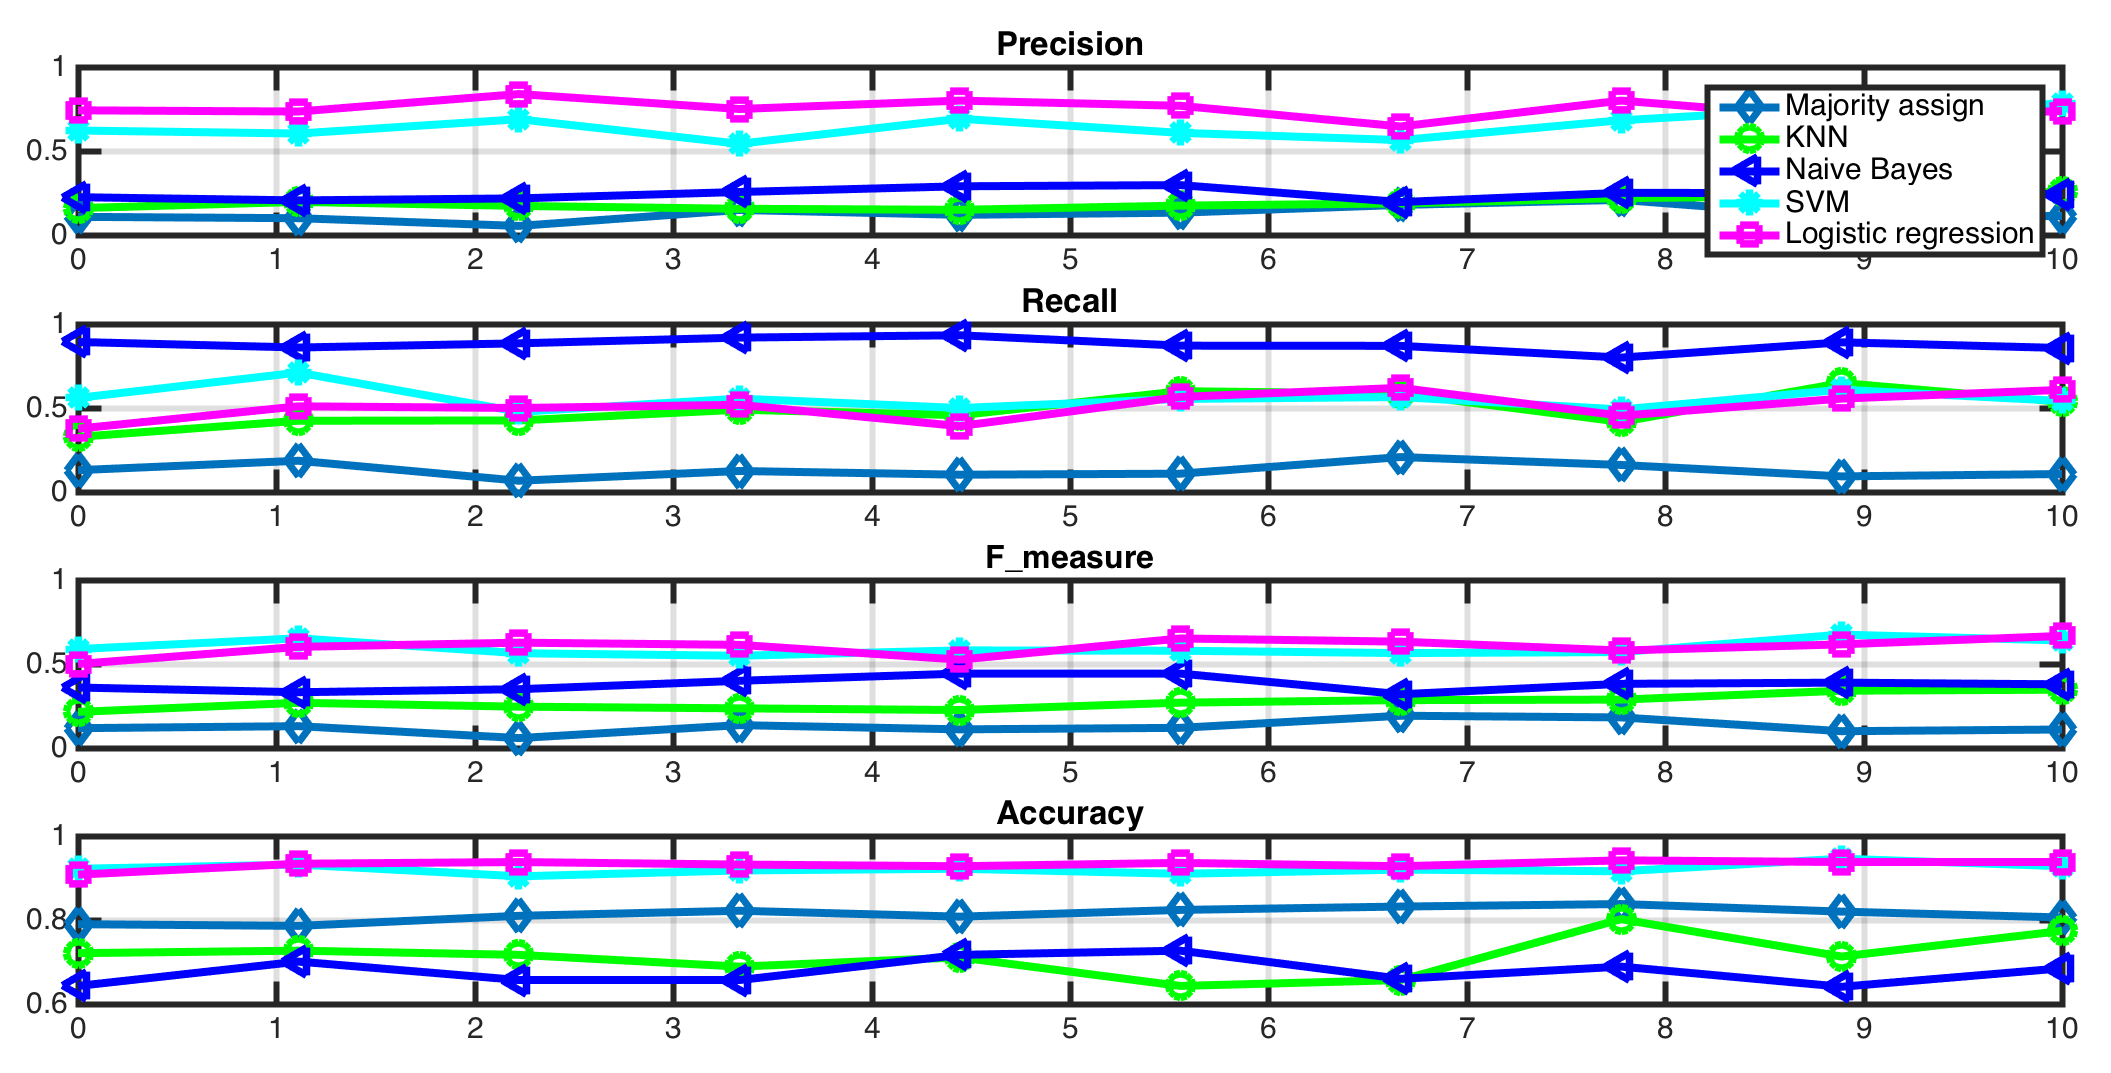
\includegraphics[width = 5in]{figures/resultsComp1.png}}
\caption{Classification methods comparison.}
\label{resultsComp}
\end{figure}

We manually labelled 1700 GSR protest records as climate or non-climate protests. Using 70\% dataset as training, and the rest 30\% as test. To ensure we have a trustworthy classification results, we evaluate the performance carefully by cross evaluation. The evaluation criteria are precision (positive predictive value), recall (true positive rate), F-measure (a measure that combines precision and recall) and accuracy (the proportion of true results both true positives and true negatives among the total number of cases examined). We compare with four well-known classification methods: majority assign, K-nearest neighbor, Naive Bayes, and weighted support vector machine (SVM). Since the climate events account for a small portion of all the events, which make it an unbalanced classification problem, so we change the traditional support vector machine into weighted SVM, by adding more importance to the climate portest events (we set the class weight to be 100). From Table~\ref{table:comparision}, we prove logistic regression method outperforms other methods uniformly.

\begin{table}[!ht]
\small
\caption{Classification methods comparison.}
\vspace{0.5em}
\centering
\begin{tabular}{|c | c | c | c | c |}
\hline
 & \textbf{Precision} & \textbf{Recall} & \textbf{F\_ measure} & \textbf{Accuracy}  \\ [1ex]
\hline
Majority assign   &  0.1274  &  0.1289 &  0.1258 &  0.8136  \\[1ex]
\hline
KNN &  0.1906  & 0.4913 &  0.2723 &  0.7154  \\[1ex]
\hline
Naive Bayes &  0.2432 & 0.8779 &  0.3798 &  0.6777  \\[1ex]
\hline
Weighted SVM &  0.6543 &  0.5565 & 0.5966 &  0.9218  \\[1ex]
\hline
Logisitic Regression & 0.7513 &  0.5102 &  \textbf{0.6018}&  \textbf{0.9322}  \\[1ex]
\hline
\end{tabular}
\label{table:comparision}
\end{table}




\section{Climate Motivated Protests}

\begin{figure}[htb]
\centerline
{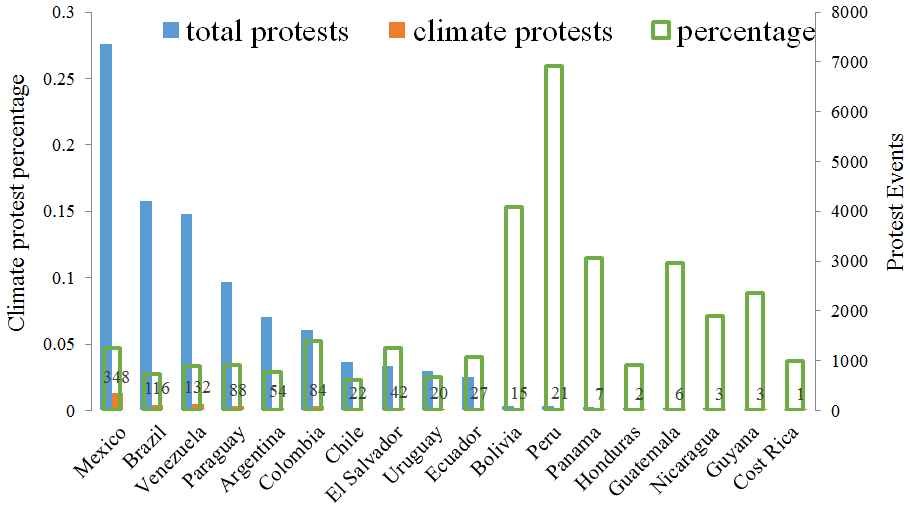
\includegraphics[width=.8\textwidth]{figures/month-country-protest3}}
\caption{Blue bar shows all the GSR protest events, yellow bar shows climate related protest events, green area shows the climate protest percentage over all the Latin American countries, from July 2012 to March 2015.}
\label{month_percentage}
\end{figure}


There were a total of 25352 recorded civil unrest events in Latin American countries from July 2011 to March 2015 that were included in our dataset.
Using our climate protest classifier, we were able to separate out protests directly or indirectly resulting from a major climatic, severe weather, or environmental event.
In the subsequent analysis, these three categories of event types are labeled with a common definition of ``climate event''.
Of the candidate civil unrest events, 991 (3.9\%) events are classified as climate-motivated across all Latin American countries for that time period.
In the subsequent sections, we conduct a multi-dimensional analysis of these protests to understand potential implications of the breadth of impact resulting from climate motivated protests.

\subsection{Frequency Analysis by Country}
The first analysis we conduct is a comparison of the representative number of protests within and across each country.
The results of our classifier selection show the total number of protests and the percentage of those that are climate motivated in Figure~\ref{month_percentage}.
The country with the most protests overall is Mexico, and Costa Rica has the least.
A similar trend is also seen in terms of climate motivated protests.
As evidenced by the climate to non-climate protest ratio, the portion of protests related to climate remains fairly constant across countries with the exception of Peru.
In this particular case, there were numerous protests centered on mining and its effect on the environment that dominate the overall protest landscape.
As the number of total protests decrease, we see more variability in the ratio as expected.
For these countries, which typically have smaller populations, the significance of a single type of protest has more of an impact on the measure than larger countries.


\begin{figure}[t]
	\centering
	\subfigure[]{
		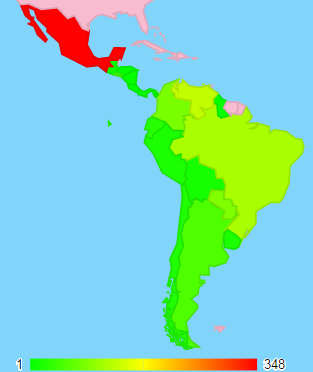
\includegraphics[height=2in] {figures/map-climate-number.png}
		\label{map_number}
	}
	\subfigure[]{
		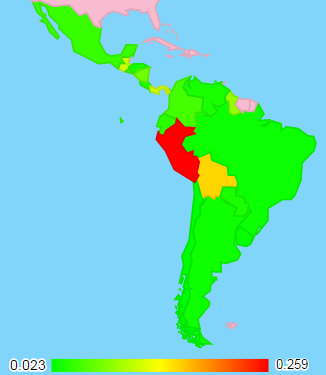
\includegraphics[height=2in] {figures/map-climate-percentage.png}
		\label{map_percentage}
	}
	\caption{(a) Climate related protests events numbers; (b) Climate related protests percentage in Latin American countries, from July 2012 to March 2015. }
\label{map}
\end{figure}



\begin{figure}[t]
\centerline
{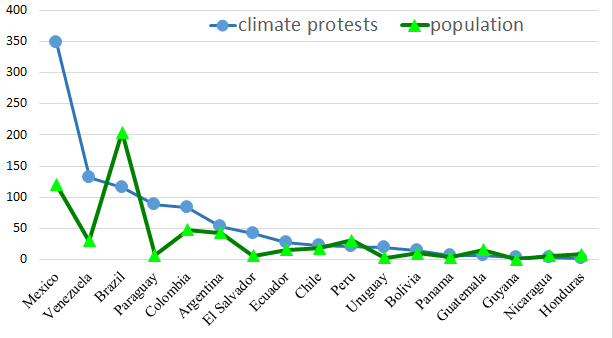
\includegraphics[width=.5\textwidth]{figures/protest-population}}
\caption{Climate protest events and population (million) of each country. The two series have a Pearson correlation coefficient 0.64.}
\label{protest-population}
\end{figure}

To show the effect of the population on the number of climate protests, we plot the result of a linear regression in Figure \ref{protest-population}.
The result of this shows an $R^2 = 0.64$, showing a slight linear relationship.
However, the interesting part of this analysis lies in the residual errors.
The set of countries including Mexico, Venezuela, Paraguay, and Colombia, all demonstrate the occurrence of more climate protests than would be expected given the entire dataset.
On the contrary, Brazil has fewer climate protests given the size of their population.
There could be a number of reasons for these findings such as socio-political stability, environmental sensitivity, and the type of climate events.
All of these are potential avenues for further causal or anecdotal studies.
In the following, however, we choose Brazil, Mexico, and Venezuela for further analysis into overall trends of climate protests, and how these are shaped in the data recovered by the classifier.


\begin{figure}[ht]
\centerline
{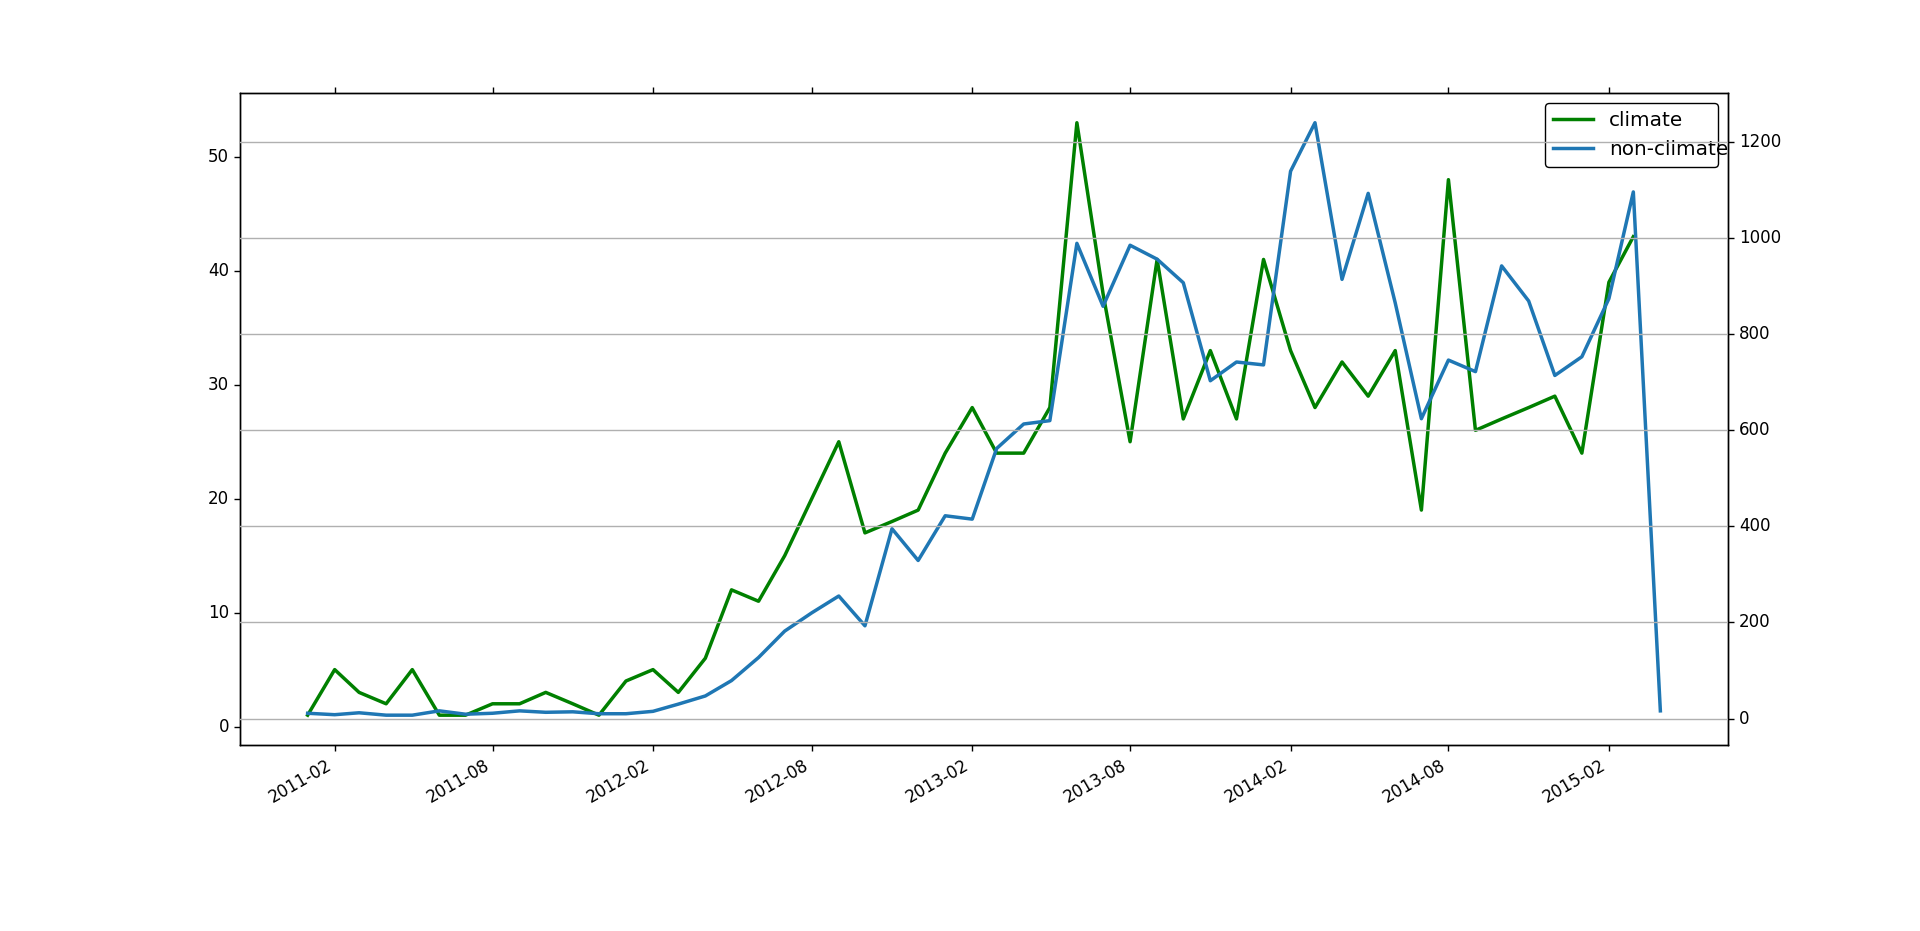
\includegraphics[width=5in]{figures/protest_time_series.png}}
\caption{climate protest and non-climate protest time series from 2011 to March 2015.}
\label{protest_time_series}
\end{figure}


We investigate the protest event time series in South American. As shown in Figure~\ref{protest_time_series}, on average, February, June, July, and August see the most climate-related protest events. We can also see the for the none-climate protest, the temporal distribution is different since it see most protests in March.


\subsection{Spatial Distribution of Climate Motivated Protests}
\begin{figure*}[t]
	\centering
    \subfigure[Mexico]{
		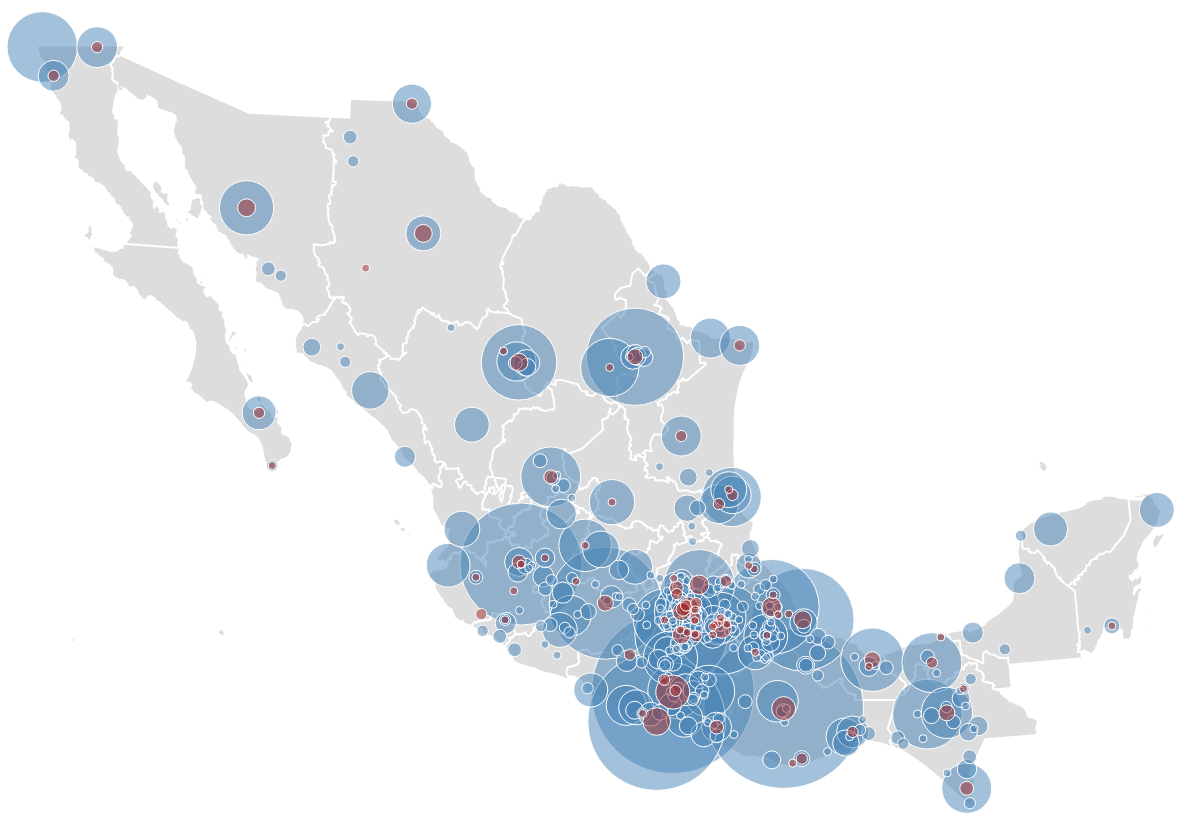
\includegraphics[height=1.6in] {figures/Mexico_climate_non-climate.png}
		\label{Mexico_map}
    }
	\subfigure[Brazil]{
		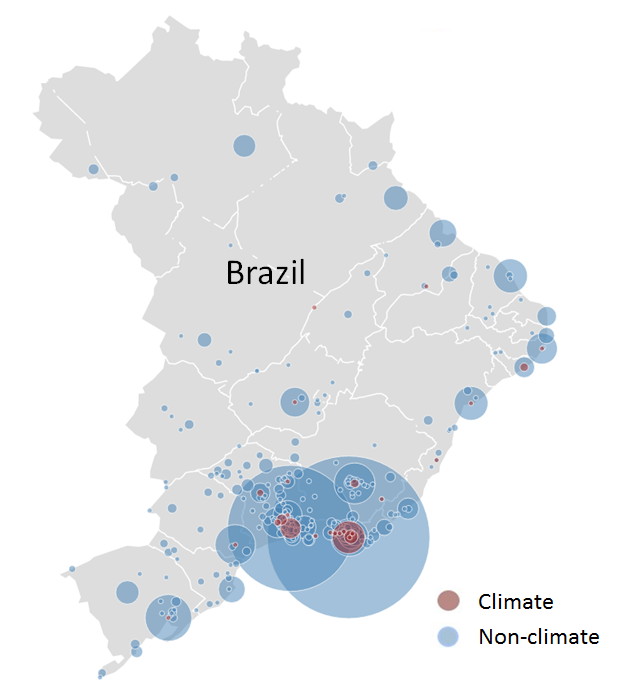
\includegraphics[height=1.8in] {figures/Brazil.png}
		\label{Brazil_map}
	}
	\subfigure[Venezuela]{
		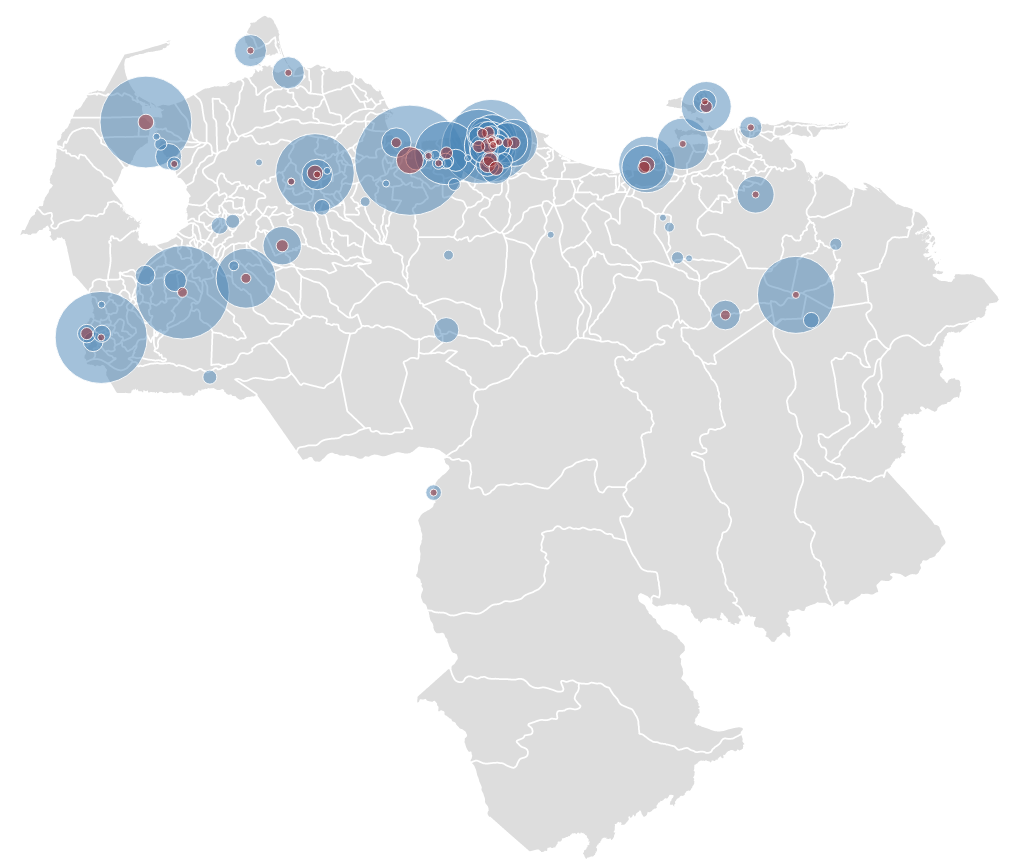
\includegraphics[height=1.7in] {figures/Venezuela_climate_non-climate.png}
		\label{Venezuela_map}
	}
	\caption{Climate and non-climate protests from July 2012 to March, 2015. Red circle represents climate related protest events, and blue circle represents non-climate related protests. }
\label{climate-map}
\end{figure*}

In this manuscript we are defining the climate protest as being different from a regular civil-unrest event by a relation to an climate event.
Next, we investigate if there is any fundamental difference in terms of where these protests occur in relation to protests in general.
For this analysis we use Mexico, Brazil, and Venezuela which all have many protest events, and the percentage of those that are related to the climate are all at about 4\%.
The spatial distribution of events is shown in  Figure~\ref{climate-map}.
Both the total number of protests and those that are climate motivated are shown and represented by the size of the blue and red shaded circles, respectively.

In both Brazil and Venezuela, many of the protests appear at or near their coastal boundaries, and Mexico has more inland activity.
However, we have already established a connection between population and protests.
This is no different for the spatial distribution, where much of the population of Brazil and Venezuela is located in coastal regions.
The protests in Brazil mainly center at two major cities Sao Paulo and Rio de Janeiro.
In Mexico and Venezuela climate protests have a more uniform distribution across the cities.
Therefore, there is no particularly strong evidence to suggest that certain regions of these countries are more prone to protest with respect to the climate than they would normally be willing to protest in general.
In terms of the climate events defined in this study, effects of climate, the environment, and extreme weather are not regionally exclusive to certain populations.
Through complex channels such as food supply, the effects of climate impact can ripple across spatial networks.



\begin{figure*}[t]
	\centering
	\subfigure[Mexico]{
		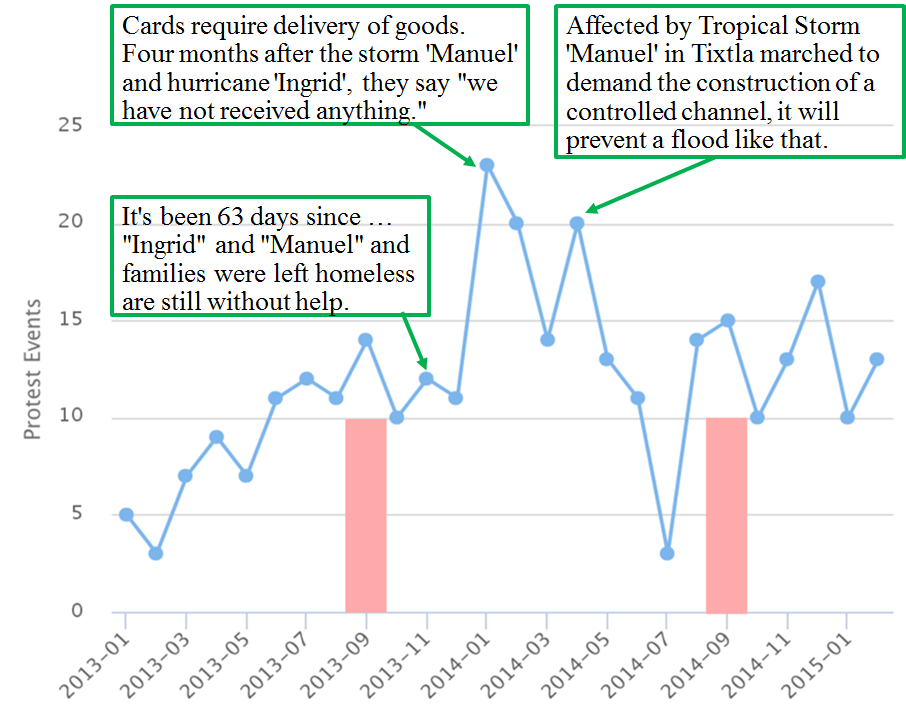
\includegraphics[height=1.3in] {figures/Mexico_disaster2.png}
		\label{Mexico_disaster_timeseries}
	}
	\subfigure[Brazil]{
		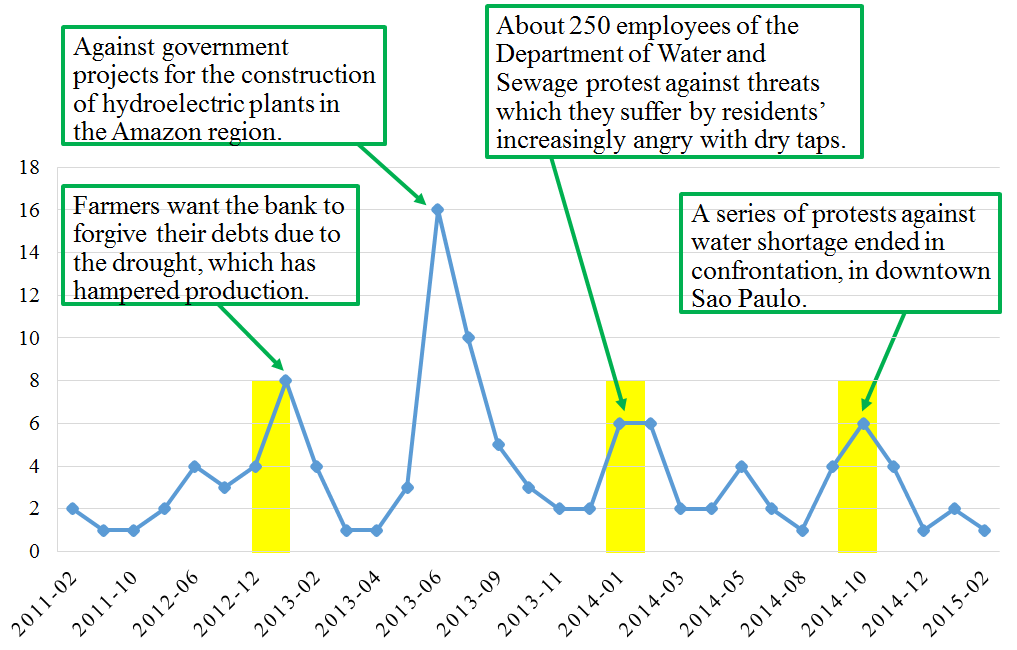
\includegraphics[height=1.3in] {figures/Brazil_disaster1.png}
		\label{Brazil_disaster_timeseries}
}
	\subfigure[Venezuela]{
		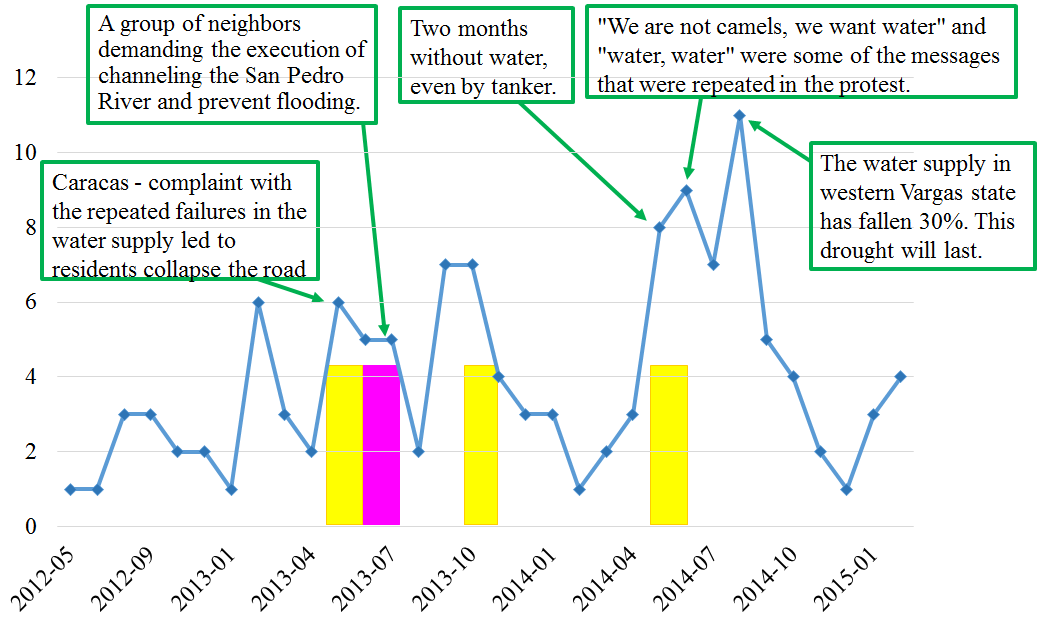
\includegraphics[height=1.3in] {figures/Venezuela_disaster.png}
		\label{Venezuela_disaster_timeseries}
	}
	\caption{(a) Mexico climate disasters and climate protests. The blue time series shows the climate related protest events, and light red vertical lines show two storm diasters in Mexico, storm Manuel in September 17, 2013 and hurricane Odile in September 15, 2014 respectively. (b)Brazil climate disasters and climate protests. The blue time series shows the climate related protest events, and yellow vertical lines show three drought diasters in Brazil, drought in Feb 2012, Heat wave in Feb 2014, and drought in Oct 2014, respectively. (c) Venezuela climate disasters and climate protests. The blue time series shows the climate related protest events, and rose vertical line show local area flood diaster, and yellow vertical lines drought disasters.}
\label{climate-timeseries}
\end{figure*}



\subsection{Temporal Dependency on Climate Events}
The temporal dependency of climate protest occurrences is analyzed for each country.
As with the spatial domain, the effects of climate events are non-local in time in some cases.
The ground truth for the events was established for extreme weather only, as the event itself is more local in time than climate and environmental changes.
This data is available by combining the following sources: International Disaster Database EMDAT\footnote{http://www.emdat.be/database}, World Disasters Timeline\footnote{http://www.mapreport.com/} and European Commission's Humanitarian Aid and Civil Protection department (ECHO)\footnote{http://ec.europa.eu/echo/}.
The official climate disaster report for each country is shown with climate related protests in Figure~\ref{climate-timeseries}.



\begin{figure}[t]
	\centering
	\subfigure[Storm Manuel, Sept 2013]{
		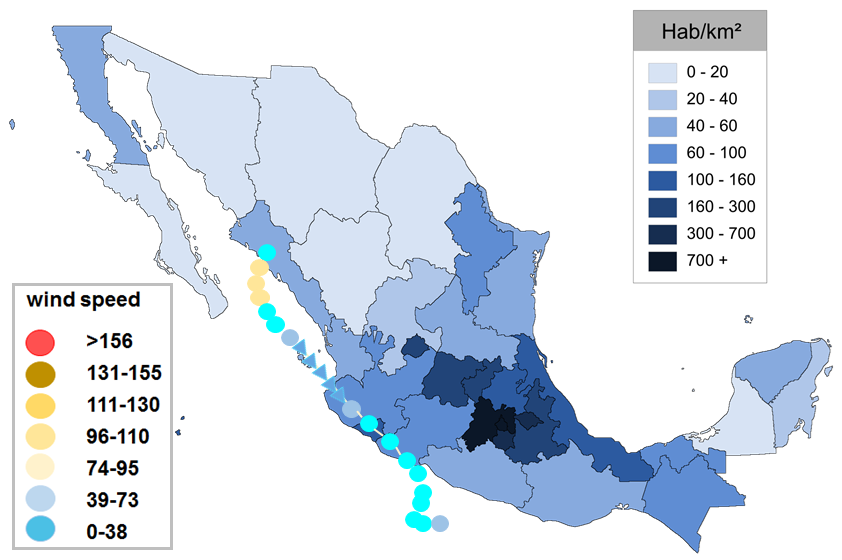
\includegraphics[width=2.5in] {figures/Mexico-2013-Manuel-new}
		\label{storm2013}
	}
	\subfigure[Hurricane Odile, Sept 2014]{
		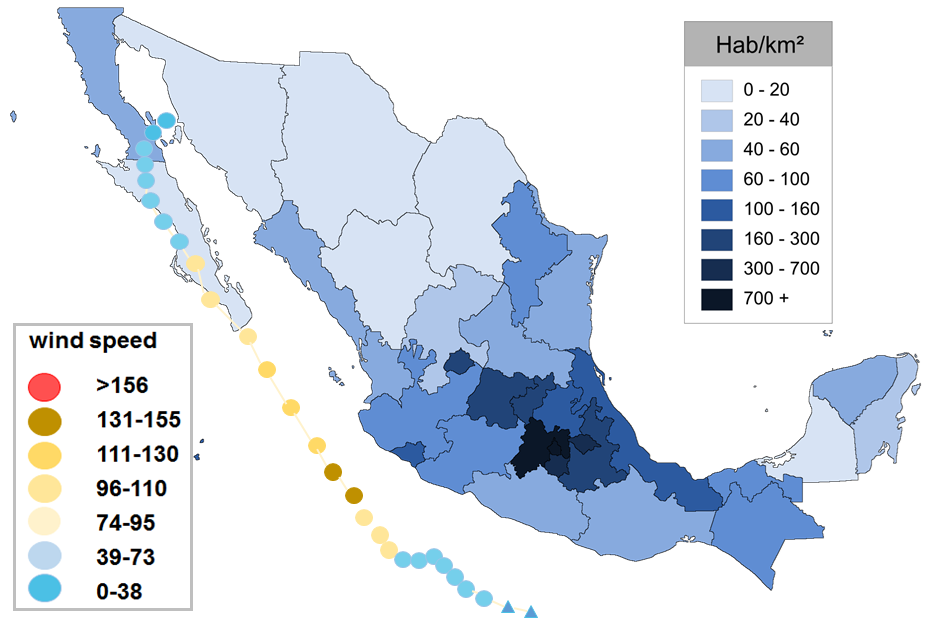
\includegraphics[width=2.5in] {figures/Mexico_2014_Odile-new}
		\label{storm2014}
	}
	\caption{The map shows population density of all Mexico's 32 states. The track shows Tropical Storm Manuel of 2013 and Hurricane Odile of 2014, points in different color represent the wind speeds. }
\label{Mexico-track-map}
\end{figure}



\paragraph{Mexico climate disasters}
Figure~\ref{Mexico_disaster_timeseries} shows the Mexican extreme weather events and protests where the blue time series represents the climate protests events, and the two red bars shows the occurrence of two storms.
The first storm is the combined tropical storm Manuel (category 1) and hurricane Ingrid in September 17, 2013.
The track maps can be seen in Figure~\ref{storm2013}.
Tropical storm Manuel crossed the west coast of Mexico and resulted in more than 23,000 people fleeing their homes due to heavy rains spawned by what had been Hurricane Ingrid.
Of those displaced 9,000 went to emergency shelters.
In terms of infrastructure, at least 20 highways and 12 bridges had been damaged\footnote{https://weather.com/storms/hurricane/news/tropical-storm-manuel-hurricane-ingrid-hit-mexico-opposite-coasts-20130916}.
After the storm, related protests and other civil unrest events broke out and lasted for more than 17 months because the government's response had been inadequate.
The storm related protests reached a climax in January 2014, and second climax in April 2014.
On November 19, 2013, there was report saying ``it's been 63 days since the onslaught of `Ingrid' and `Manuel' and families were left homeless are still without help''\footnote{Quotes are translated from the native language of the country.}
Four months after the storm Manuel and the effects of Hurricane Ingrid, they say ``we have not received anything''.
On April 7, protest descriptions said ``Affected by Tropical Storm `Manuel' in the municipal head of Tixtla marched to demand the construction of a controlled channel, it will prevent a flood like that caused the overflow from the Black Lagoon in September 2013''.
The last protest event we have on record from the climate protest classifier occurred 17 months after the original event.
This demonstrates that the residual capacity of these events to impact the livelihoods of people is not guaranteed to be local in time.
As we show, the range of impact can extend even beyond the occurrence of other storms.

\begin{figure}[t]
\centerline
{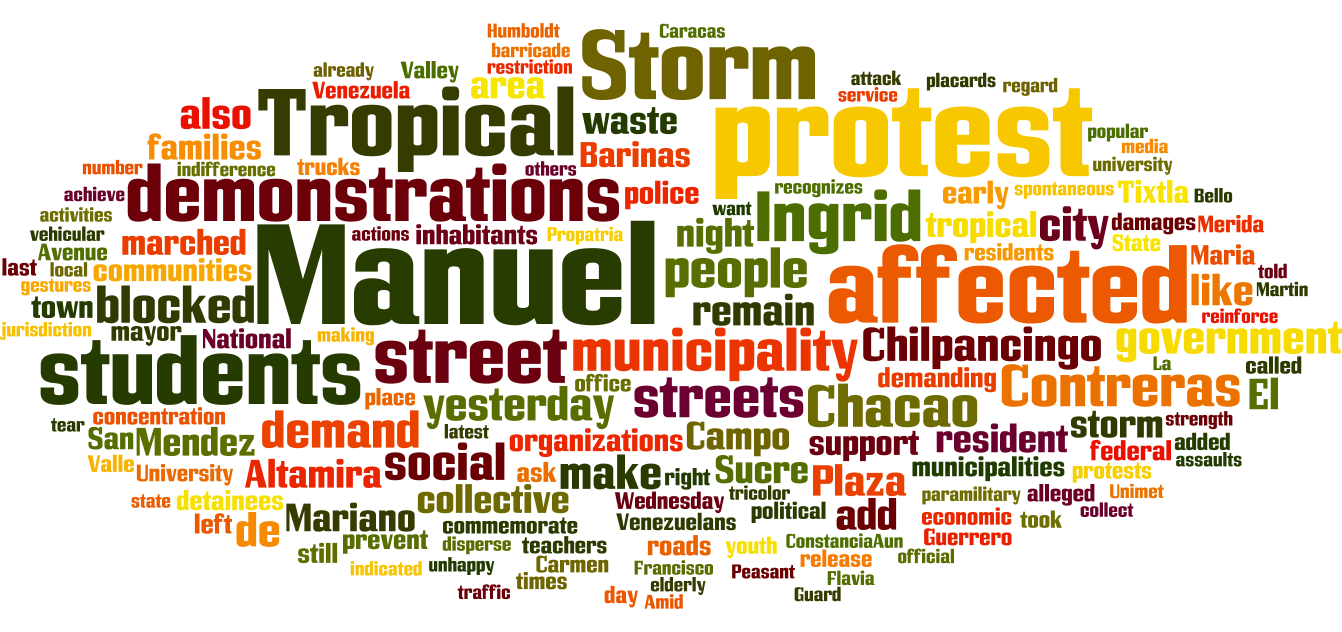
\includegraphics[width=3in]{figures/Mexico_Manuel_wordcloud.png}}
\caption{Word cloud of Mexico storm Manuel, Sept 13, 2013.}
\label{Manuel_word_cloud}
\end{figure}



In Figure~\ref{Mexico_disaster_timeseries}, the second red bar shows hurricane Odile.
It is a category 3 storm that occurred in 2014, and the track of the storm's path is shown in Figure~\ref{storm2014}.
Despite hurricane Odile being a more intense storm, there were not many protests related to the event.
Comparing the storm's paths in Figure~\ref{Mexico-track-map}, Tropical Storm Manuel hit Mexico's mainland, which caused more  destruction.
Hurricane Odile 2014 had less of an impact on the Mexican mainland, even though it crossed the state of Baja California. However, this is the second smallest Mexican state by population.
This can explain why storm 2013 lead to tremendous protests, while hurricane 2014 does not.


\paragraph{Brazil climate disasters}
Figure~\ref{Brazil_disaster_timeseries} shows the relationship between protests classified by our algorithm and actual extreme weather events in Brazil.
The three yellow bars show three separate drought events in Brazil, which resulted in drought related protests almost immediately.
The drought in February 2012 hampered production, which caused farmers to protest.
The heat wave in February in 2014, and drought in October 2014 resulted in water shortages, causing civil unrest.
The biggest spike in June 2013 described protests against government's projects for the construction of hydroelectric plants in the Amazon region\footnote{http://www.bloomberg.com/news/articles/2013-06-05/protests-over-brazil-hydropower-leads-to-delays-and-boosts-costs} and is more of an environmental impact type of event.
In general, for these events we see predominantly local relationships in time between the protest and the preceding event.
For Brazil in particular, the extreme weather event matches fairly well with the onset of drought.


\paragraph{Venezuela climate disasters}
In Figure~\ref{Venezuela_disaster_timeseries}, the climate motivated events are shown in relation to relevant extreme weather events for Venezuela.
The pink bar represents sudden onslaught of rain in June 2013 that caused a heightened risk of flooding and landslides in the densely populated communities on the outskirts of Caracas.
It triggered a small portion of protests to prevent flooding.
The yellow bars denote drought disasters.
The drought in May 2014 triggered rationing of tap water in the capital, Caracas, where residents formed lines lasting hours to fill jugs of water\footnote{http://www.breitbart.com/national-security/2014/05/31/severe-scarcity-prompts-venezuelan-government-to-ration-water/}.
This drought disaster lasted so long that related protests reached a climax in September 2014.
Unlike Brazil, the data in Venezuela on droughts proved tough to ascribe to a particular drought event.
They occur rather frequently and there is a substantial amount of overlap in the residual protest events that it was difficult to distinguish to which it was referring.


\section{Climate protests causality}
\begin{figure}[ht]
\centerline
{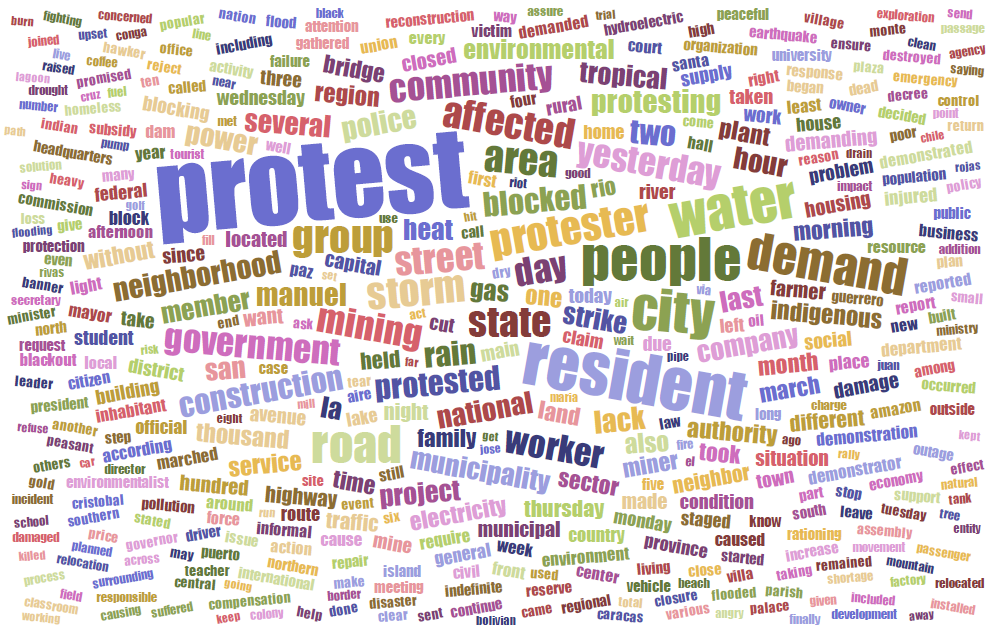
\includegraphics[width=4in]{figures/Climate_word_cloud.png}}
\caption{Word cloud of all the climate related protests, from GSR descriptions.}
\label{wordcloud}
\end{figure}

\subsection{Word cloud}
Of the climate related protests, we are interested in what are the protesters demanding. To have a birds view of climate protests, we extract all the climate protest descriptions and plot the word cloud, as shows in Figure~\ref{wordcloud}. We can see words like `water', `storm', `mining', `rain', `construction', `power', `heat', `gas', `environment', `electricity', and other weather, environment related keywords are dominant, which gives us a general idea of what protesters are demanding.

\begin{figure}[t]
\centerline
{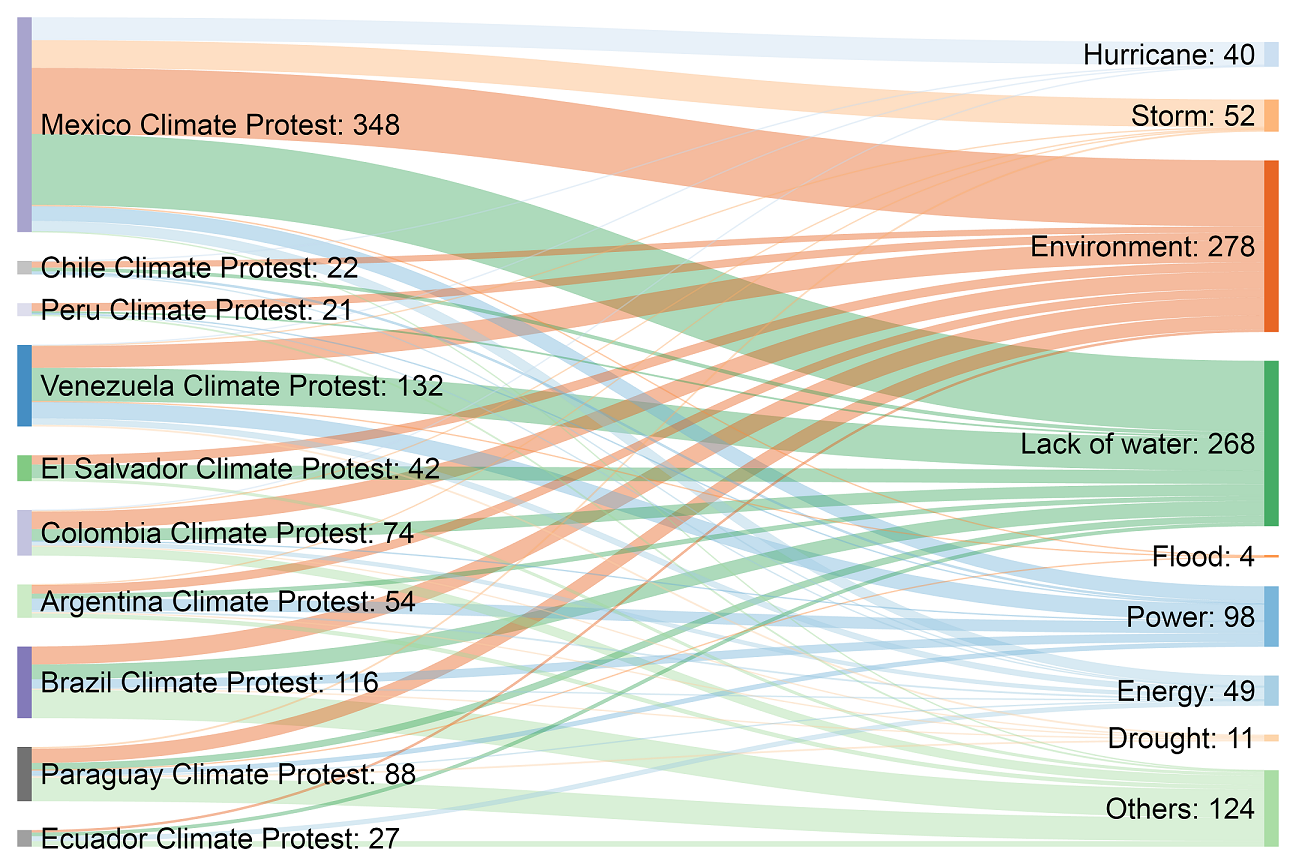
\includegraphics[width=4in]{figures/causality1.png}}
\caption{Climate protest causality diagram. Left bar shows ten countries' climate protest numbers, and right bar shows nine climate event categories which cause climate protests.}
\label{causality}
\end{figure}

\subsection{Analysis of Protest Descriptions}
As stated previously, we are not blind to the realization that the causes of climate motivated protests are in general complex.
In the following, we analyze the descriptions of the protest events in order to gain insight into the general pathways by which protests within our corpus have occurred.
Shown in Figure~\ref{causality} is a weighted Sankey diagram showing the bipartite graph of the most common keywords in the descriptions of protests from each country.
Apparently, many of the protests identified by the classifier in one way or another have something to do with lack of water followed by climateal effects in general.
Other prominent keywords include mentions of power and energy issues.
Each country also exhibits its own protest keyword categories.
In Mexico, the most notable protest keywords involve are lack of water, environmental concern, storm and hurricane.
In Venezuela, apart from lack of water and environment problems, the dominant keywords are blackout and energy issues.
In Peru, more than half of climate protests are about a mining project, which is an environment concern.
While in Argentina, 35\% events protest against blackout issues.
We expand on these observations in the following where we analyze several dimensions of the keywords to extract details about pathways to protest.


\begin{figure}[ht]
	\centering
	\subfigure[Mexico]{
		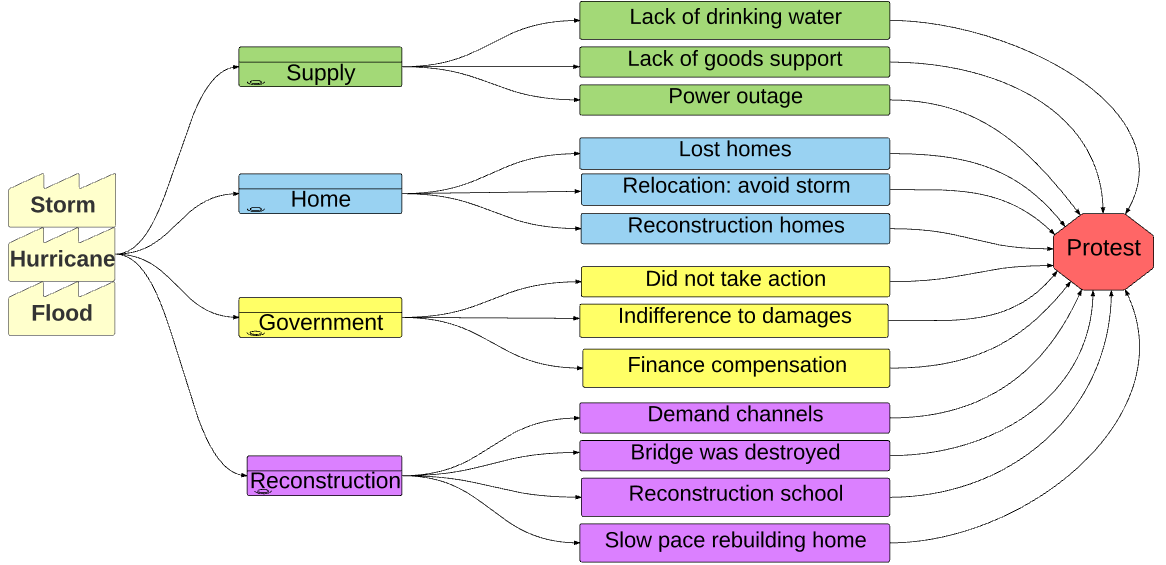
\includegraphics[width=5in, height=2.4in] {figures/Mexico-diagram2.png}
		\label{Mexico_causality}
	}
	\subfigure[Brazil]{
		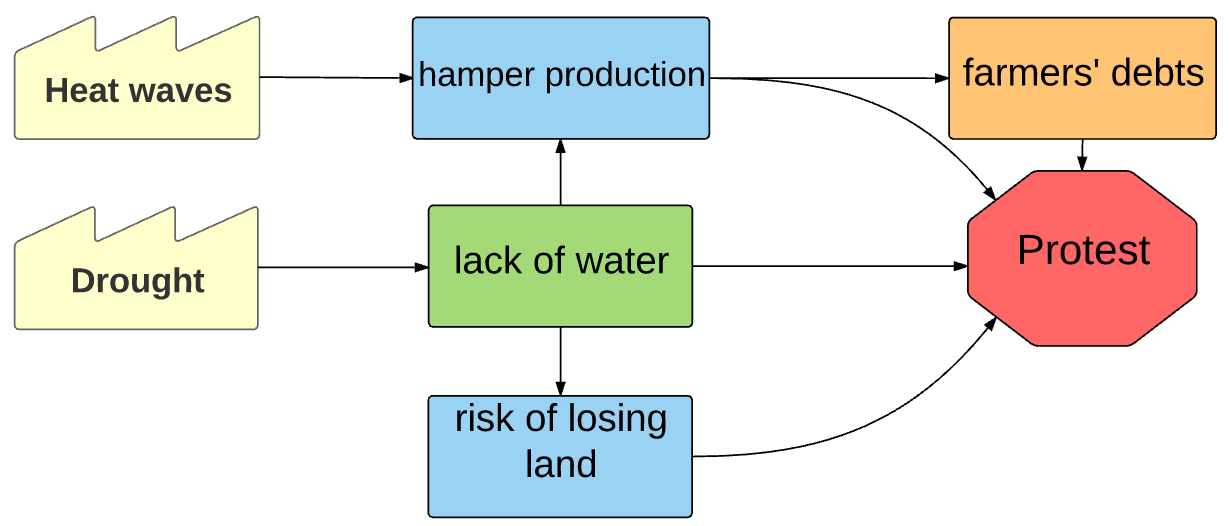
\includegraphics[width=3in, height=1.5in] {figures/Brazil-diagram.png}
		\label{Brazil_causality}
	}
    \subfigure[Venezuela]{
		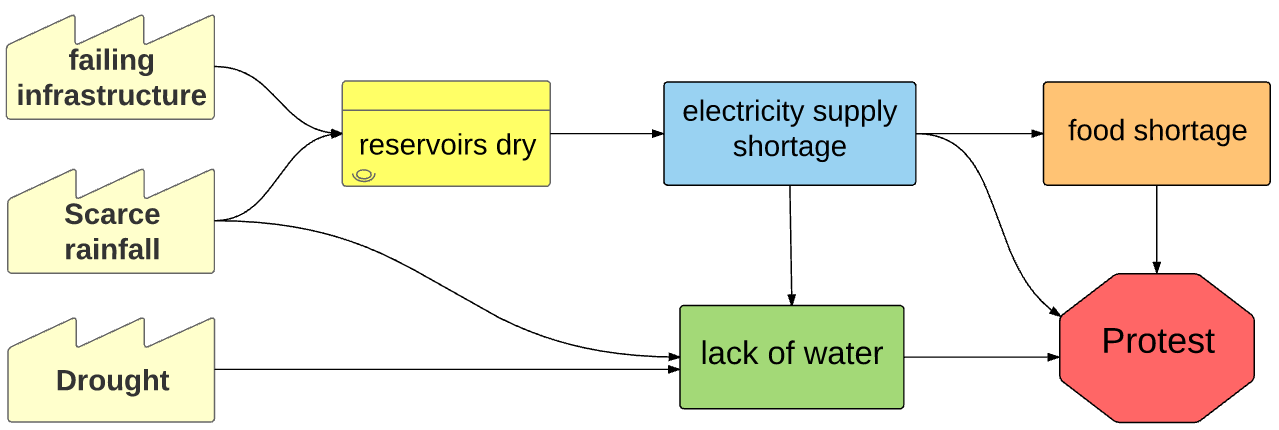
\includegraphics[width=3in, height=1.5in] {figures/Venezuela-diagram2.png}
		\label{Venezuela_causality}
    }
	\caption{Climate protest causality diagram}
\label{three-causality}
\end{figure}




\begin{figure*}[t]
	\centering
	\subfigure[Brazil]{
		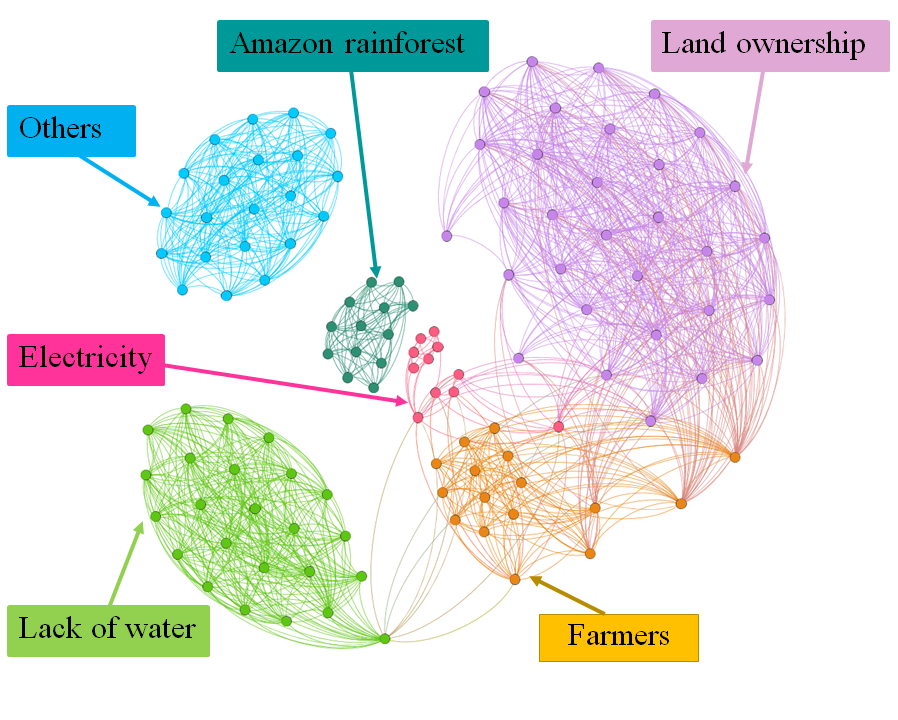
\includegraphics[width=2in, height=1.4in] {figures/Brazil_cluster.png}
		\label{Brazil_cluster}
	}
    \subfigure[Mexico]{
		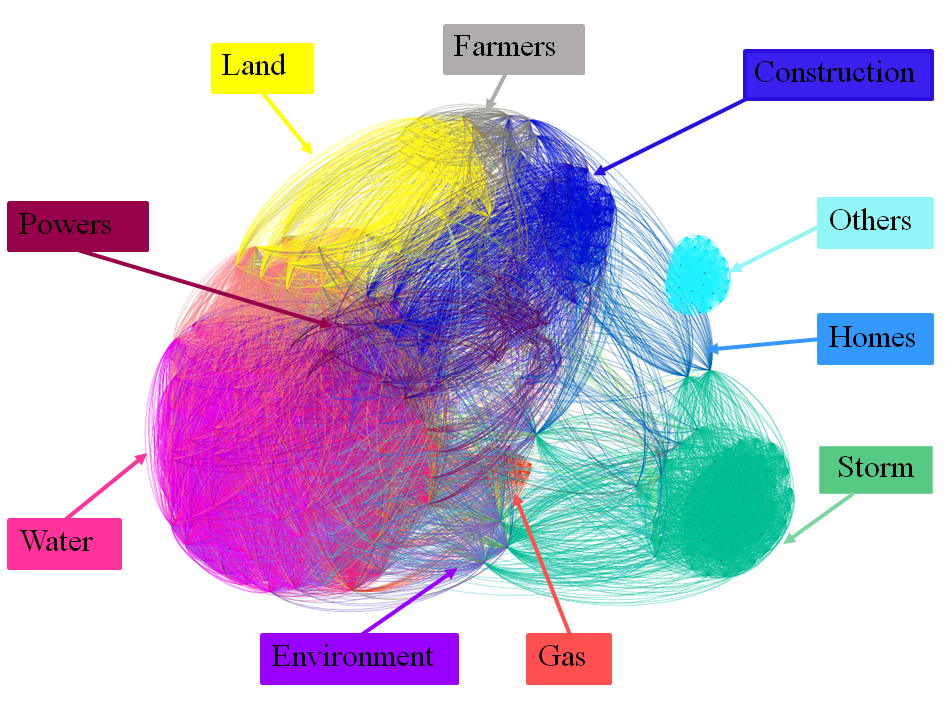
\includegraphics[width=2in, height=1.4in] {figures/Mexico_cluster1.png}
		\label{Mexico_cluster}
    }
	\subfigure[Venezuela]{
		\includegraphics[width=2in, height=1.4in] {figures/venezuela-cluster2.png}
		\label{Venezuela_cluster}
	}
	\caption{Climate protest clustering results}
\label{clusters}
\end{figure*}


\subsection{Pathways to Climate Motivated Protest}
%For some severe and dominant climate events, such as storm, hurricane, flood, and drought events, we employ the knowledge graph to represent the link relationships between entities. By matching the object or subject with climate related keywords, and predicate to be causality relationship like result of, cause by, lead to, blamed, accused of, demanding, against, request, we can locate and further identify the causality of most protest descriptors. Specifically, the causality analysis is based on three steps, as described following.

To determine the different pathways to climate motivated protest events, a three step process was implemented to extract the relevant information.

\textbf{a. Text enrichment.}
Messages with textual content (Tweets, Newsfeeds, Blog postings, etc.) are subjected to shallow linguistic processing prior to analysis. Applying BASIS technologies' Rosette Language Processing (RLP) tools, the language of the text is identified, the natural language content is tokenized and lemmatized and the named entities identified and classified. Finally, messages are geocoded with a specification of the location (city, state, country), being talked about in the message.

\textbf{b. Knowledge graph construction.}
In the scope of this study, an entity network is a graph $G(E, R)$ where entities $E = {e_1,
. . ., e_n}$ can be linked to one another through relationships $R = {r_1, . . ., r_n}$ defined by conceptual interactions, and thus called a knowledge graph. knowledge graphs are used to represent its logic based on semantic networks.
How to represent knowledge and extract entities and their relationship from text?
The general extraction patterns rule is Noun Phrase - Verb Phrase - Noun Phrase. We can also employ multilingual rules for phrase patterns learnt using association mining based on collocations. Using an open source, GraphDb (Neo4j) to store and query knowledge triples.
%Neo4j is a very robust, scalable solution for Knowledge representation, which provides an expressive query language : CYPHER, and a framework for implementing graph theoretic search algorithms.
The general scheme is Subject - Predicate - Object. Subject is a concept, which can be person, organization, location, event, noun phrase; Predicate can be either a verb action or (predefined) relation type; Object can be either a concept or (some) value. With all the enriched articles as input, since their named entities and verb phrases being identified and classified, the system can automatically extract the structural knowledge and load them into Graph database. It worths to note the entities may evolve along space and time.

\textbf{c. Causality query.}
With a complete knowledge database, we are going to poses domain specific questions, for example, who are the main players in the article? what are the reasons for the protest? To such questions like that, we are seeking causal (base) relations between concepts. Specifically, we are interested in entities to be storm, hurricane, heat, draught, etc,, climate related keywords. By matching the object or subject with climate related keywords, and predicate to be causality relationship like result of, cause by, lead to, blamed, accused of, demanding, against, request, we can locate and further identify most of protest causalities.

Figure~\ref{Mexico_causality} shows the storm caused protests demands in Mexico, which generally falls into four categories: supply, home, government and reconstruction. In the supply related protest, the causality includes but not limited to: lack of drinking water, lack of good support, and power outage. The second category is about home, they protest either because of lost homes, or request to relocate to avoid storm, or request to reconstruct homes. Another protest type targets at government, they either fight because government did not take action, or blame government's indifference to damages, or request finance compensation to the damages. In the reconstruction category, residents demand reconstruct channels to avoid more storms, request to reconstruct bridges, roads, schools, or unsatisfied with the slow pace of rebuilding homes. Figure~\ref{Brazil_causality} describes the causality of Brazil climate related protests. One line is heat wave hampered production, which cause farmers' protests, the other line is drought causing residents lack of drinking water thus lead to protest, and the third line is lack of water causing farmers facing the risk of losing land, which result in protest. In Venezuela, the protests are more water-electricity centralized, as shown in Figure~\ref{Venezuela_cluster}. Scarce rainfall, drought plus failing infrastructure, which makes water shortage and blackout is an everyday fact of life in Venezuela. The electricity shortage deteriorates water shortage, leads to food shortage, and worsens food quality, and so forth. All those situation touches off climate related protests.


\section{Climate protest pattern}
The above analysis shows the general protest causality, however, we intend to further discover the coherent correlations of protest reasons, hoping to answer questions like is there any protest pattern, or are there some protests associate with others.
We treat each protest event as a node and connect two nodes with weight based on their protest description text similarity. Specially, we pay attention to the protest themes or protest demands, if two descriptions have the same protest demanding, their weight will be very high, otherwise, their connection weight tends to be 0. In this way, we build a weighted undirected network $G(V, E, W)$, with each protest as node $V$, and their connection as edge $E$, their weight as $W$. If the weight between two nodes is 0, there will be no edge. We employ Louvain method~\cite{blondel2008fast} to split the network into several clusters.


We show in Figure~\ref{clusters} the climate protest clustering results that provides the protest proportion and coherent correlations among different protest types. Figure~\ref{Brazil_cluster} illustrates Brazil's climate protest pattern, the results shows that in Brazil, the largest protest cluster is about land ownership which accounts for 26.7\%, the second cluster lack of water takes up 20.7\%, farmers cluster occupies 13.8\%, of which, one interesting discover is land and farmers clusters are closely coherent, and lack of water is also closely bind with farmers. Amazon rainforest is another striking protest which is responsible for 11.3\%. Figure~\ref{Mexico_cluster} shows the protest pattern of Mexico, which has the most climate protest events and complex patterns. We can see the rose red cluster which denotes lack of water is the most dominant protest, accounts for 20.5\%, the green cluster represents tropical storm is the second largest protest type, takes up 19.0\%, the dark blue cluster construction accounts for 17\%, and the yellow cluster land is responsible for 11.8\%. We find, water protest is intertwined with environment protest and power protest, land protest is closely related with farmers, while construction cluster is coherent with baby blue cluster which denotes homes (2.6\%). Figure~\ref{Venezuela_cluster} gives the overview clustering results of Venezuela climate protests. We can see, the yellow cluster which represents lack of water protests takes up the largest portion, as high as 55.8\%, the green cluster which denotes power outage accounts for second part, 22.1\%, and the blue cluster which stands for gas shortage accounts for 5\%, the purple cluster shows the rest climate protest portion, which include food shortage, medicine shortage, water tank robbery behavior, etc.. Clearly, as expected, lack of water protest is intertwined with power outage protest, which corresponds to the fact that lack of water and power shortage is everyday life in Venezuela.


\section{Climate protests in Twitter}
We are also interested in climate events influence on social media, such as Twitter. Using keywords list we are able to filter tweets, then cluster tweets into different partitions based on similarity among tweets using distance function, taking tweets content, geolocation and other features into consideration.

Events Clustering is used to separate events happened at same place or at same time, or the separate different events happened simultaneously on local and entire country. By measure the distance among tweets based on similarity, tweets collection can be clustered into subsets in which tweets are exactly related and similar. Each partition includes similar tweets stand for a specific event. Without events clustering, different events will be mixed. As shown in Figure~\ref{Mexico-events}, Mexico Hurricane were mixed with severe drought happen in Culiacan, with the aid of event clustering, we are able to distinguish those distinct extreme weather events, even though they may happen at the same time. For each event, we plot the related Tweets word cloud besides the flag. Figure~\ref{Brazil-events} illustrates four drought events in Brazil, on May 2012.

\begin{figure}[th]
	\centering
	\subfigure[Mexico]{
		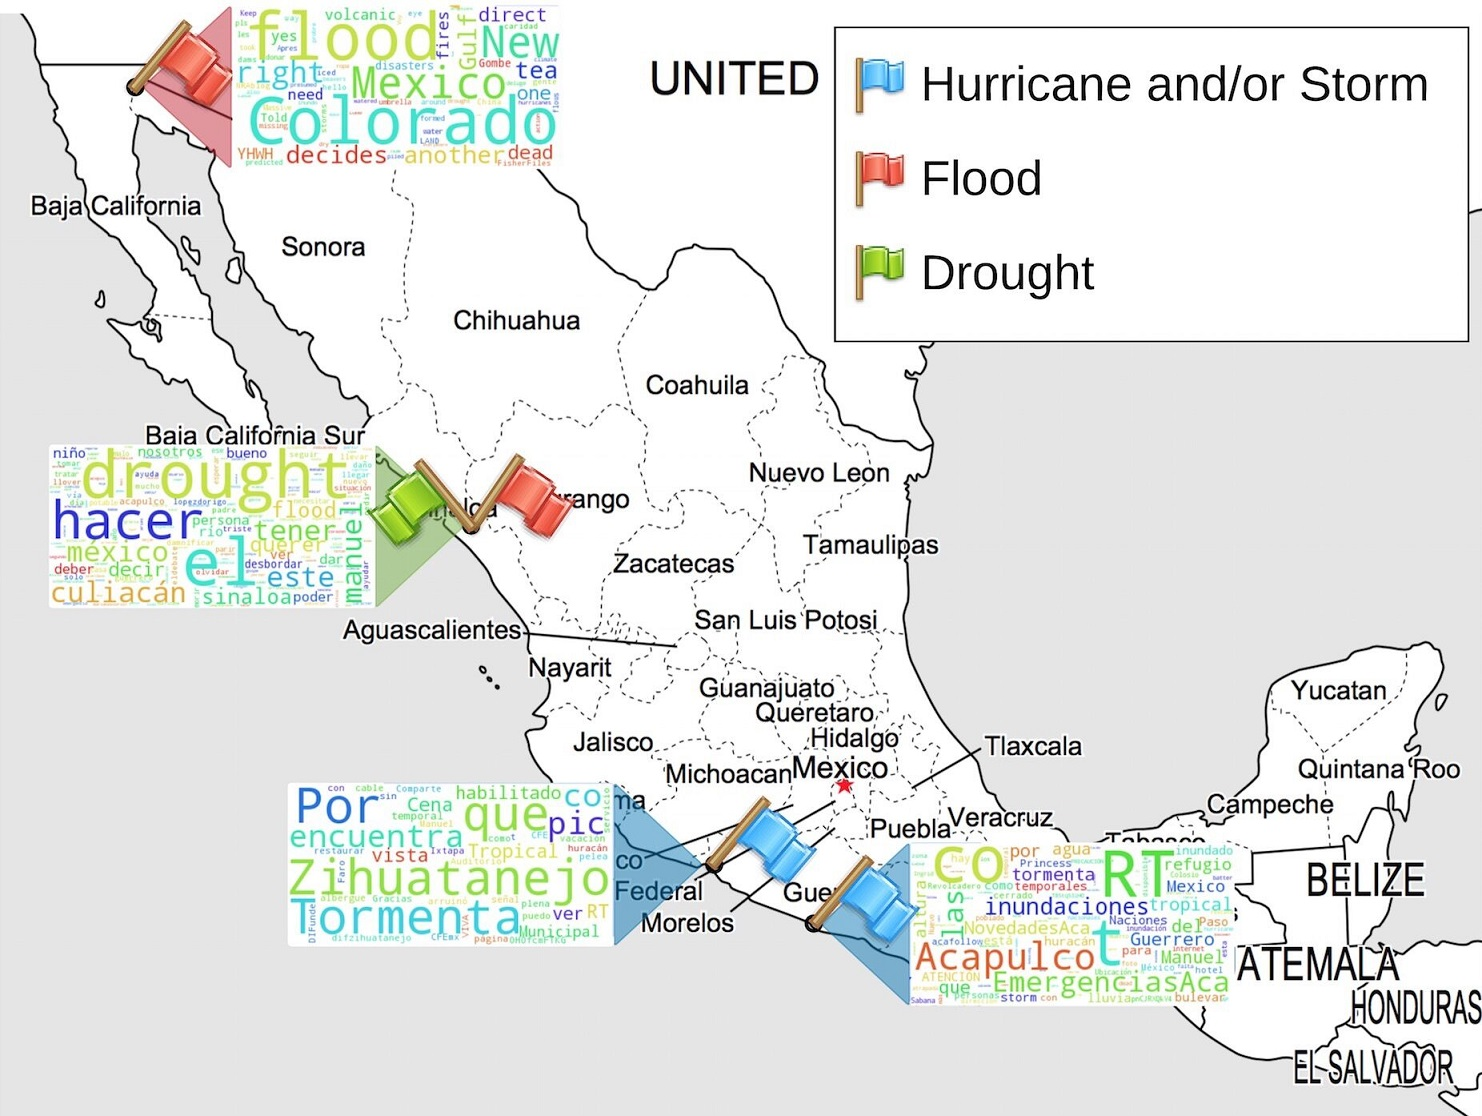
\includegraphics[width=2.5in, height=2in] {figures/Mexico-events.jpg}
		\label{Mexico-events}
	}
	\subfigure[Brazil]{
		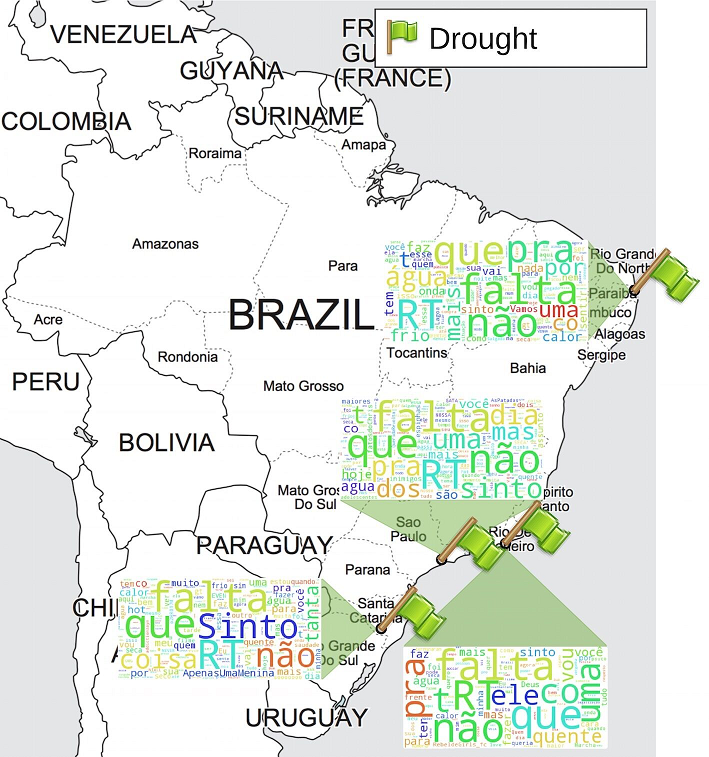
\includegraphics[width=2.5in, height=2in] {figures/Brazil-events.jpg}
		\label{Brazil-events}
	}
	\caption{Climate protest events in Mexico, Sept 2013 and Brazil, May 2012. Different flag represents different climate disasters. The adjacent world cloud shows Twitter discussion as per that event. }
\label{Twitter-events}
\end{figure}


\section{Discussion}
Climate changes, extreme weather and environmental catastrophes can all exert a devastating amount of harm to people around the world.
To better understand this process, we show different pathways to protest following severe events in Latin America from 2011 to 2015.
Our analysis differs from those previously published in that we consider the breadth of climate protests over a wide spatial and temporal domain.
This is accomplished by identifying climate related protests using a logistic regression classifier acting over keyword vectors of protests descriptions in our protest GSR dataset.
We found this approach achieved an F-score of 0.60 and accuracy of 0.93, which was the best preforming of other common binary classifiers.
The results of the classifier indicate a number of broad properties about climate related protests.

From our analysis, we found different climate diasters may cause related protests with different time span, for instance, the Mexico storm Manuel aroused climate related protest as long as 17 months, while in Venezuela, the protests caused by one drought always overlap with the other drought. This paper discloses protest causalities in Latin American countries, illustrate the pathways from climate disasters to climate protests. This paper also identifies the climate related protest patterns, discover the coherent relationship among different protests demanding, such as in Venezuela, the majority protests are against lacking of water, which has high co-occurrence with protests against power outage.





%GSR event defines six different protest event types according to the concerns of people involved, they are employment, housing, energy \& resources, economic polices, other government policies, other. We are interested to see which event type is most dominant of all the climate related protest events. We plot the event type distributions for each country in Figure~\ref{fig:climate_eventType}.
%
%\begin{figure}[t]
%	\centering
%	\subfigure[Argentina]{
%		\includegraphics[width=3in,height=1.8in] {figures/climate/Argentina_type.png}
%		\label{fig:type_Argentina}
%	}
%	\subfigure[Brazil]{
%		\includegraphics[width=3in,height=1.8in] {figures/climate/Brazil_type.png}
%		\label{fig:type_Brazil}
%	}	
%	\subfigure[Chile]{
%		\includegraphics[width=3in,height=1.8in] {figures/climate/Chile_type.png}
%		\label{fig:type_Chile}
%	}
%	\subfigure[Colombia]{
%		\includegraphics[width=3in,height=1.8in] {figures/climate/Colombia_type.png}
%		\label{fig:type_Colombia}
%	}
%	\subfigure[El Salvador]{
%		\includegraphics[width=3in,height=1.8in] {figures/climate/Elsd_type.png}
%		\label{fig:type_Elsd}
%	}
%	\subfigure[Mexico]{
%		\includegraphics[width=3in,height=1.8in] {figures/climate/Mexico_type.png}
%		\label{fig:type_Mexico}
%	}
%	\subfigure[]{
%		\includegraphics[width=3in,height=1.8in] {figures/climate/Paraguay_type.png}
%		\label{fig:type_Paraguay}
%	}
%	\subfigure[]{
%		\includegraphics[width=3in,height=1.8in] {figures/climate/Venezuela_type.png}
%		\label{fig:type_Venezuela}
%	}
%	\caption{Event type distribution of climate events for South American.}
%\label{fig:climate_eventType}
%\end{figure}


%
%\begin{figure}[th]
%	\centering
%	\subfigure[]{
%		\includegraphics[width=3in,height=1.95in] {figures/climate/Argentina_percentage.png}
%		\label{fig:percentage_Argentina}
%	}
%	\subfigure[]{
%		\includegraphics[width=3in,height=1.95in] {figures/climate/Chile_percentage.png}
%		\label{fig:percentage_Chile}
%	}
%	\subfigure[]{
%		\includegraphics[width=3in,height=1.95in] {figures/climate/Colombia_percentage.png}
%		\label{fig:percentage_Colombia}
%	}
%	\subfigure[]{
%		\includegraphics[width=3in,height=1.95in] {figures/climate/Urugauy_percentage.png}
%		\label{fig:percentage_Urugauy}
%	}
%	\caption{Compare GSR events, climate events and climate events percentage of South American.}
%\label{fig:climate_percentage}
%\end{figure}
